\documentclass[11pt, oneside]{article} 
\usepackage{geometry}
\geometry{letterpaper} 
\usepackage{graphicx}
	
\usepackage{amssymb}
\usepackage{amsmath}
\usepackage{parskip}
\usepackage{color}
\usepackage{hyperref}

\graphicspath{{/Users/telliott_admin/Tex/png/}}
% \begin{center} 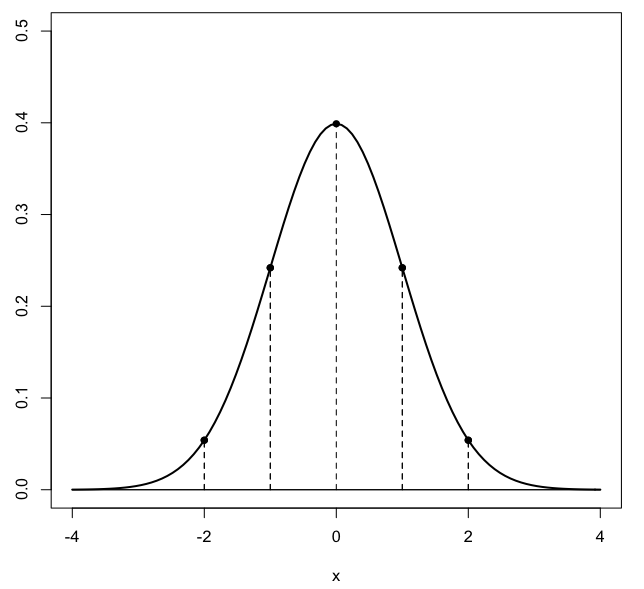
\includegraphics [scale=0.4] {gauss3.png} \end{center}

\title{Taylor Series --- Shankar}
\date{}

\begin{document}
\maketitle
\Large

Suppose we have a function $f(x)$, but 
\begin{quote}"imagine that you don't have access to the whole function.  You cannot see the whole thing.  You can only zero-in on a tiny region."\end{quote}

around $f(0)$, where you know the value.  So the question is, what do we guess the function will do near $f(0)$?  
 
The first approximation is that
\[ f(x) \approx f(0) \]
We really can't say anything more.  $f(0)$ is the best guess for what the value of the function is (we're talking about continuous and continuously differentiable functions).

Now suppose we know the slope of the function at $0$, $f'(0)$.  Then, since $\Delta y = f'(0) \Delta x = f'(0) x$, we can get a better approximation as the linear approximation:
\[ f(x) \approx f(0) + f'(0)\ x + \dots \]

For most functions, there will be more terms.  If $f$ is not a linear function, then the slope won't be constant.  So 

\begin{quote}"the rate of change itself has a rate of change .. the second derivative."\end{quote}  

The term we are going to add is
\[ f''(0)\ \frac{x^2}{2} \]
so
\[ f(x) \approx f(0) + f'(0)\ x + f''(0)\ \frac{x^2}{2}  + \dots \]

A simple way to see why we have $x^2/2$ is to take derivatives on both sides.  The terms like $f'(0)$ and $f''(0)$ are constants, they have been evaluated at $x=0$. The first derivative is
\[ f'(x) \approx  f'(0) + f''(0)\ x  + \dots \]
We evaluate at $x=0$ and the term $f''(0)\ x$ goes away because of the $0$ multiplying the constant $f''(0)$.  So we have just
\[ f'(x) \approx  f'(0)  \]
and that matches. Now take the second derivative
\[ f''(x) \approx  f''(0) \]
and that matches too.  We can see a pattern here.  

The fourth term is
\[ f(x) \approx f(0) + f'(0)\ x + f''(0)\ \frac{x^2}{2!}  + f'''(0)\ \frac{x^3}{3!} + \dots \]

You might not be expecting the factorial which I snuck in there.  But if you go back to the exercise above, where we evaluated derivatives, you can see why it works.  When we take the first derivative 
\[ \frac{d}{dx} (f'''(0)\ \frac{x^3}{3!}) =  f'''(0)\ \frac{x^2}{2!}\]
the $3$ comes down from the power and then turns $3!$ in the denominator into $2!$.  The next derivative will bring down the $2$.  So everything cancels properly.  

If you like $\Sigma$ notation, we can write
\[ f(x) = \sum_{n=0}^{\infty} f^n(0) \frac{x^n}{n!} \]
with the understanding that $0! = 1$.  The approximation is better the closer $x$ is to $0$, and the more terms the better as well.  

There is one final wrinkle to this derivation.  The series can be modified deal with $x$ near any value $a$, not just near $0$.  The modification is
\[ f(x) = \sum_{n=0}^{\infty} f^n(a) \frac{(x-a)^n}{n!} \]
This is the Taylor series.  The series near $a=0$ is known as the Maclaurin series.

\subsection*{1/1-x}
The first example is
\[ f(x) = \frac{1}{1-x} \]
We know the answer to this.
\[ \frac{1}{1-x} = 1 + x + x^2 + x^3 \]
Proof:
\[ 1 = (1-x)(1 + x + x^2 + x^3) \]
Multiplying by $1$, the second term $x$ is matched by $-x$ from the first term in the multiplication by $-x$, and so on.  The whole thing vanishes, leaving just $1$.

We want to evaluate $f(x)$ near $0$, let's say, at $x=0.1$.  The correct value of the function is
\[ f(x) = \frac{1}{0.9} = 1.11111 \dots \]

Let's try to approximate using the series.  We need derivatives
\[ f(x) = \frac{1}{1-x} \]
\[ f'(x) = \frac{1}{(1-x)^2} = (1-x)^{-2} \]
\[ f'(0) = 1 \]
so the linear approximation is
\[ f(x) \approx 1 + 1x = 1.1 \]

For the next term we obtain
\[ f''(x) = 2(1-x)^{-3} \]
The $2$ is cancelled by the $2!$ in the denominator, so this cofactor is $1$ and we're left with
\[ f''(0)\ \frac{x^2}{2} = x^2 = 0.01 \]
And I think we can see where this one is going.

However, you probably remember that this series
\[ \frac{1}{1 - x} = 1 + x + x^2 + x^3 + \dots \]
diverges for $|x| \ge 1$, and the Taylor series does too.

The morale of the story is that for some series, there is a radius of convergence and the series is only valid for $x$ within that radius.

\subsection*{binomial}\

Another very useful series is the binomial.
\[ f(x) = (1 + x)^n \]
\[ f(0) = 1 \]
\[ f'(0) = n(1 + x)^{n-1} = n \]
\[ f''(0) = n(n-1)(1 + x)^{n-2} = n(n-1) \]
So the series is
\[ (1 + x)^n \approx 1 + nx + n(n-1) \frac{x^2}{2} \]

We use this one a lot.

A nice application is relativistic energy
\[ E = mc^2 f \]
\[ f =  1/\sqrt{1-\frac{v^2}{c^2}} \]
This is, in disguise, a binomial with $n=-1/2$ and $x=-v^2/c^2$ so the expansion is
\[ f  \approx 1 + nx = 1 + \frac{v^2}{2c^2} \]
so the energy is 
\[ E \approx mc^2 (1 + \frac{v^2}{2c^2} ) \]
And we see that the second term is just the kinetic energy, $mv^2/2$.

\subsection*{exponential, sine and cosine}
Let's take a look at $e^x$.  The nice thing about $e^x$ is the first derivative, in fact all the derivatives, are just $e^x$, and since we're evaluating them at $0$, all those factors become $1$.  So the series is just
\[ e^x = \sum_{n=0}^{\infty} \frac{x^n}{n!} = 1 + x + \frac{x^2}{2!} + \frac{x^3}{3!} + \dots \]
Let's try sine and cosine.  

Cosine first
\[ f'(0) = -\sin(x) \bigg |_{x=0} = 0 \]
\[ f''(0) = -\cos(x) \bigg |_{x=0} = -1 \]
\[ f'''(0) = \sin(x) \bigg |_{x=0} = 0 \]
\[ f''''(0) = \cos(x) \bigg |_{x=0} = 1 \]

So the pattern is, every other term, with alternating signs.
\[ \cos x = 1 - \frac{x^2}{2!} + \frac{x^4}{4!} + \dots \]
The sine function loses the first term (because $\sin 0 = 0$), then we have the same pattern of every other term and alternating sign.
\[ \sin x = x - \frac{x^3}{3!} + \frac{x^5}{5!} + \dots \]


\subsection*{one more}
Finally, we'll sneak in an oddball.  Suppose we consider
\[ f(x) = e^{ix} \]
where $i = \sqrt{-1}$.  Let's just follow the rules and see where we get to.  First of all, the derivatives look like this
\[ f'(x) = ie^{ix} \]
\[ f''(x) = i^2e^{ix} = -e^{ix} \]
\[ f'''(x) = i^3e^{ix} = -ie^{ix} \]
\[ f''''(x) = i^4e^{ix} = e^{ix} \]
Evaluated at $x=0$, the exponentials become $1$ and we are left with the pattern $1, i, -1, -i \dots$.  So our series is
\[ e^x = 1 + ix - \frac{x^2}{2!} - i\frac{x^3}{3!} + \frac{x^4}{4!} + i\frac{x^5}{5!} - \frac{x^6}{6!} - i \frac{x^7}{7!} \dots \]
\[ = \cos x + i \sin x \]

These series then lead to definitions of the sine and cosine in terms of the exponential:
\[ e^{ix} = \cos x + i \sin x \]
\[ e^{-ix} = \cos (-x) + i \sin (-x) = \cos x - i \sin x \]
Add
\[ e^{ix} + e^{-ix} = 2 \cos x  \]
or subtract
\[ e^{ix} - e^{-ix} = 2i \sin x \]
So
\[  \frac{d}{dx} (2 \cos x) = \frac{d}{dx} ( e^{ix} + e^{-ix}) = i( e^{ix} - e^{-ix}) = i(2i \sin x) = - 2 \sin x \]
\[  \frac{d}{dx} (2i \sin x) = \frac{d}{dx} ( e^{ix} - e^{-ix}) = i( e^{ix} + e^{-ix}) = i(2 \cos x) \]

\end{document}  